\section{Implementierung}

\subsection {Inbetriebnahme Greifarm}
Der OMX wird als Bausatz geliefert.Für die Inbetriebnahme ist daher der Zusammenbau und die Installation der entsprechenden Software  nötig. 
\subsubsection{Zusammenbau}
-Bausatz ca 40 Teile (ohne Schrauben)\\
-Rausbrechen Plastik bei Vorbereitung Servos\\
-Servos einzeln anschließen und per Dynamixel Wizard ID setzen\\
Der Bausatz des OMX besteht aus ca. 60 Teilen (ohne Schrauben, s. Abbildung \ref{fig:omxparts}).Einige der mit den Servomotoren mitgelieferten Teile werden dabei nicht benötigt, da der Bausatz des OMX diese auch enthält oder ersetzt (z.B. längere Kabel). Von allen Schrauben wurde außerdem Ersatz mitgeliefert.\\
Der Zusammenbau erfolgte nach der auf der Webseite verfügbaren Bauanleitung VERWEIS ANLEITUNG. Zu beachten ist, dass hier vorrausgesetzt wird, dass den Servos bereits die IDs 11 (Basis des Greifarms) bis 15 (Greifer) zugewiesen wurden. Dies kann über die Software DYNAMIXEL Wizard{\footnote{VERWEIS ODER LINK}} gemacht werden: die Servos einzeln über das U2D2{\footnote{ERKLÄRUNG ODER VERWEIS HINZUFÜGEN}} an den PC anschließen, die ID setzen und den Servo entsprechend markieren oder die ID merken. Weiterhin müssen bei den Abdeckungen der Servos 12 und 14 die vorgestanzten Abdeckungen herausgebrochen werden. Dies ist in der Anleitung leicht zu übersehen. Weiterhin wird angenommen, dass das Horn der Servos bereits angebracht ist. Hierbei ist darauf zu achten, dass die Einkerbung an Horn und Servo übereinstimmen.
\begin{figure}[ht!]
\centering
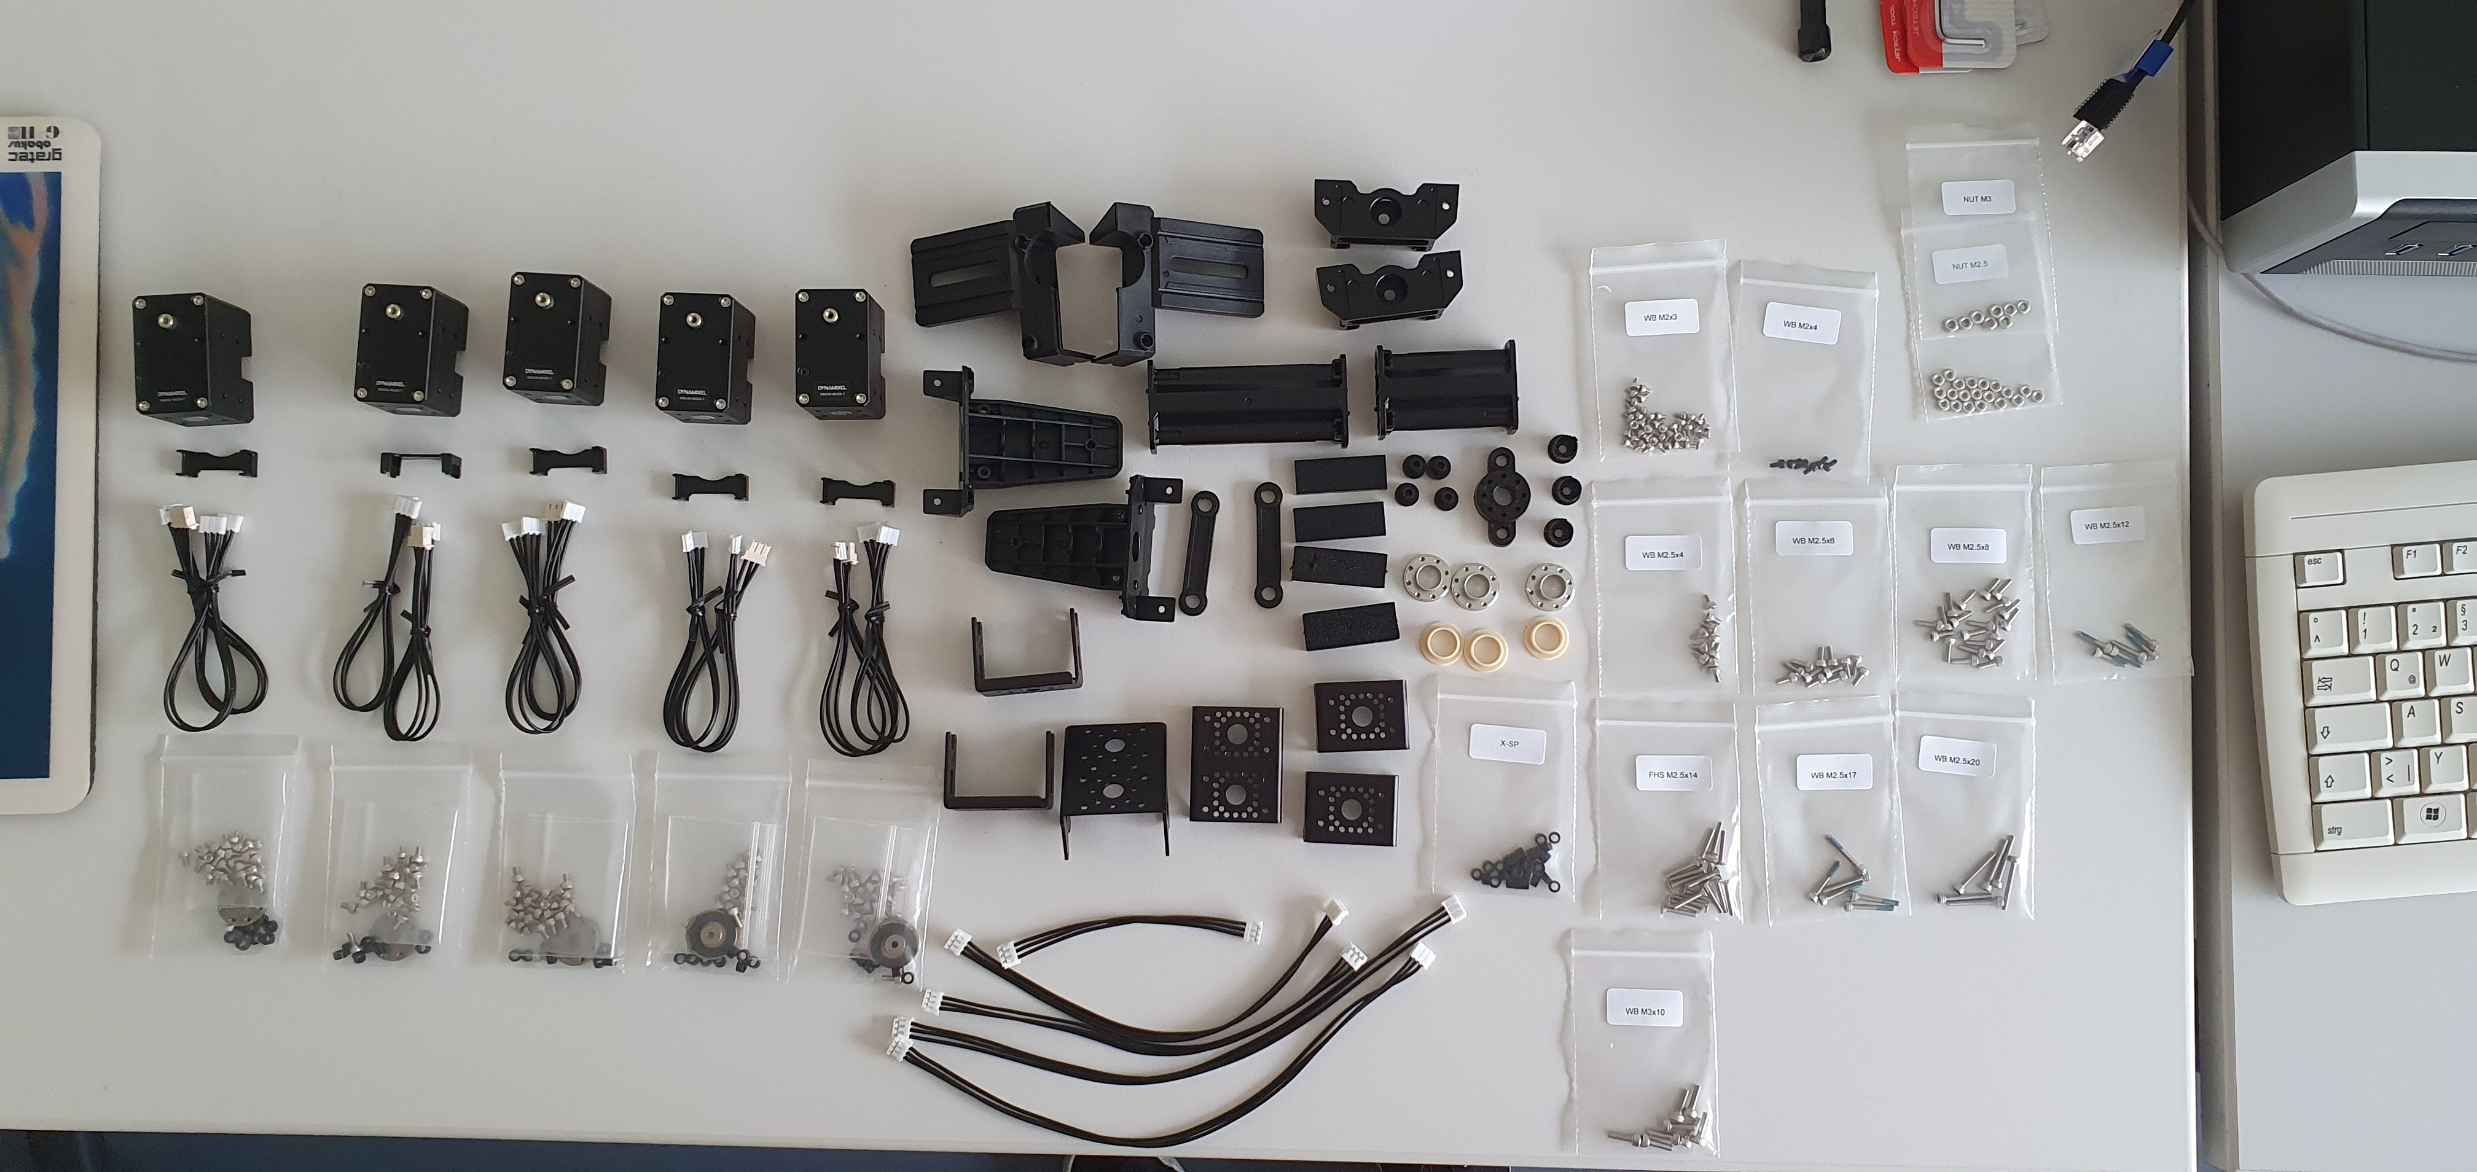
\includegraphics[width=\textwidth]{parts.jpg}
\caption{Bausatz für den OpenMANIPULATOR-X}
\label{fig:omxparts}
\end{figure}
\subsubsection{Virtuelle Maschine}
-Ubuntu 20.04\\
-- Auflösung Einstellung "keine"\\
-Installation ROS2 Foxy\\
-Installation OMX\\
Zur Nutzung des Greifarms wurde eine \ac{VM} mit VirtualBox {\footnote{https://www.virtualbox.org}} von Oracle aufgesetzt. Als Betriebssystem der \ac{VM} wurde das für ROS2 Foxy empfohlene \citep{foxyreq} Ubuntu 20.04 {\footnote{\url{https://releases.ubuntu.com/20.04/}}} gewählt. Danach wurde entsprechend der Anleitung für den OpenMANIPULATOR-X \citep{foxyinstall} zuerst ROS 2 Foxy über das Installations-Script von ROBOTIS und im Anschluss die für den Greifarm benötigten Packages installiert.
\subsection{Steuerung OMX}
Die Steuerung des OMX erfolgt über die vom \emph{open\_manipulator\_x\_controller}\\ \verb|open_manipulator_x_controller| zur Verfügung gestellten Topics und Services.
\subsubsection{OMX-Controller}
Der OMX-Controller ist ein Package, welches automatisch beim Installieren der für den OMX benötigten Software installiert wird. Er kann über die entsprechende Launch-Datei mit dem Befehl
\begin{verbatim}
ros2 launch open_manipulator_x_controller 
     open_manipulator_x_controller.launch.py
\end{verbatim}
gestartet werden.
\subsubsection{Topics}
\subsubsection{Kinematik}
\subsubsection{Teleop} \label{teleop}
Mit einem laufenden OMX-Controller kann der OMX auch ohne extra Programmierung direkt ferngesteuert werden. Mögliche Geräte zur Steuerung sind die Tastatur sowie Playstation- und XBOX-Controller. Für \ac{ROS2} Foxy wird aktuell allerdings nur die Steuerung über die Tastatur unterstützt.\\
Der OMX kann dabei sowohl im Task Space als auch im Joint Space kontrolliert werden (s. Abbildung \ref{fig:teleopkeyboard}). Zusätzlich gibt es 2 vordefinierte Posen (Init und Home) in die der OMX bewegt werden kann (s. Abbildung \ref{fig:teleiopposes}).
\begin{figure}[ht!]
\centering
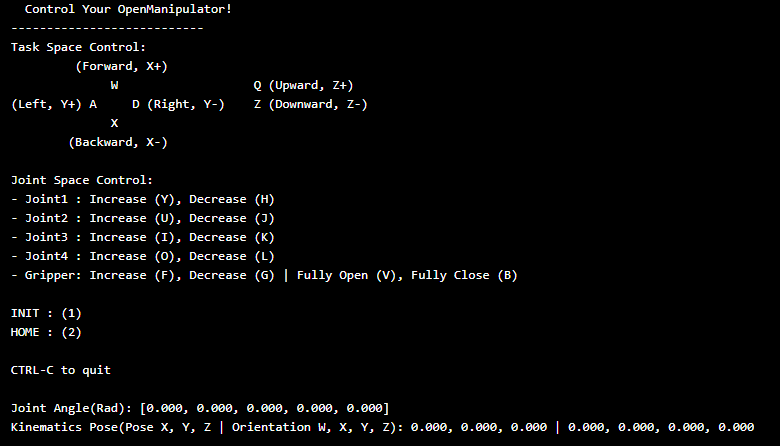
\includegraphics[width=\textwidth]{teleopkeyboard.png}
\caption{Fernsteuerung des OMX über die Tastatur}
\label{fig:teleopkeyboard}
\end{figure}
\subsection{PlanSys2}
\cite{plansys}\\
Für die Implementierung der in \ref{konzept:nodes} genannten Funktionalitäten wird das Framework \ac{PlanSys2} genutzt. Es übernimmt dabei alle Funktionalitäten: die Verwaltung der Daten zur Domäne und dem aktuellen Problem erfolget über die domain-expert und problem-expert Nodes. Die planer Node ist für die komplette Planung zuständig und die Executioner Node für die Ausführung des Plans.\\
Es müssen hier lediglich die Domäne erstellt sowie die tatsächliche Funktionalität der einzelnen Aktionen implementiert werden.
\subsubsection{PDDL-Domain}
-Durative Actions\\
-Gripper + Blockworld\\
- keine existential/negative Preconditions\\
Beim erstellen der Domäne ist zu beachten, das \ac{popf} nicht alle Funktionen unterstützt, die mit PDDL beschrieben werden können. Dies beinhaltet unter anderem existentielle sowie negative Vorbedingungen. Die vollständige Liste ist auf \ref{popfpddlsupport} zu finden. Das Wort Action im Namen der Nodes bezieht sich hier auf die Aktionen der Domäne, nicht auf \ac{ROS2} Actions.
\subsubsection{Action Nodes}
Obwohl in der Domäne mehr als 2 Aktionen beschrieben sind, beschränken sich die ausgeführten Aktionen auf ein bewegen des OMX sowie die Kontrolle des Greifers. Für diese wird jeweils eine Node erstellt. Damit diese Nodes von \ac{PlanSys2} genutzt werden können müssen sie von der Basisklasse \verb|plansys2::ActionExecutorClient| erben. Da diese von \ac{PlanSys2} nur in C++ zur Verfügung gestellt wird, müssen auch die Aktionen in C++ implementiert werden.\\
In jeder Aktion muss die Methode \verb|void do_work()| implementiert werden. Diese wird mit einem bestimmten Zeitintervall aufgerufen während die Aktion aktiv ist. Das Intervall wird im Konstruktor gesetzt (s. Zeile \ref{code:line:nodeintervall} in \ref{code:gripperactionnode}). Das Mapping einer Node zu einer Aktion erfolgt durch das Setzen des Parameters \verb|action_name| nach dem Erstellen der Node (s. Zeile \ref{code:line:actionname} in \ref{code:gripperactionnode}).
\subsubsection{Move Gripper Aktion}
\subsubsection{Control Gripper Aktion}
Die Logik Node zur Steuerung des Greifers wird in der Klasse \verb|ControlGripperAction| (s. \ref{code:gripperactionnode}) implementiert. Da es vom OMX kein Feedback gibt, ob oder wann etwas gegriffen wurde, wird die Aktion mit einer fixen Wartezeit implementiert: wenn die Aktion gestartet wird, wird ein Request zur Steuerung des Greifers erzeugt (s. Zeile \ref{code:line:gripperrequest} in \ref{code:gripperactionnode}) und gesendet und nach einer bestimmten Zeit die Aktion beendet. Um unnötige Aufrufe der Methode während des Wartens zu verhindern wird die Wartezeit über das Zeitintervall zur Ausführung der Node gesetzt. Die Aktion wird hierdurch immer beim 2. Aufruf der Methode \verb|do_work| beendet.\\
Zum Senden des Requests wird ein \ac{ROS2} Client für den Service \verb|goal_tool_control| mit dem Typ \verb|open_manipulator_msgs::srv::SetJointPosition| erstellt. 
Um sowohl die Aktionen zum Öffnen sowie Schließen des Greifers mit einer Node implementieren zu können wird ein Parameter eingeführt, welcher über die Launch-Datei gesetzt wird und die Bewegung des Greifers bestimmt.
%\newpage